The neurosciences, and more generally, brain and behavioral sciences, imply
extensive interactions among disciplines to advance our 
appreciation for the relation between brain and behavior. 
\footnote{Several important scientific projects such as The Human Brain Project are clear
illustration such interactions.}. 
The inherent challenge, however, lies in bringing together the distributed competences
of many individuals or even institutions and exchanging across interdisciplinary
borders using common techniques.  
This situation is excerbated by the technical sophistication of modern
data analysis and brain simulation, which often impedes their adoption 
in the communtiy.

These challenges call for two kinds of solutions. First, there is a need
for comprehensive, modern computational libraries written in a widely
used and available programming languages, such as MNE-Python \cite{mnepython},
a Python package for treating M/EEG data via time-frequency analyses and inverse
solutions and the Brain Connectivity
Toolbox \cite{rubinov2010complex} for analyzing the graph theoretic
properties of structural and functional connectivity. Second, there is
a need for the implementation
of collaborative infrastructure for sharing not only data, but expertise; 
CARMEN \cite{austin2011carmen} and G-Node \cite{herz2008g} are two such
examples of developing platforms for collaborative work and data sharing, 
in the domains of cellular and systems neurophysiology.
Ideally, solutions will be easily extended by its own users, as is often
the case in open source and scientific projects, due to the rapid 
evolution of use cases and requirements.

TheVirtualBrain (TVB) provides its own solutions to these two problems.  In an
initial step, they were addressed in two independent developments: one whole
brain-simulator library developped in \matlab{} and a web platform for
collaborative interactions in the context of multi-purpose data analysis which
was developed in Python.  In each case, the choice of the language was dictated
both by the scientific context and the technical constraints. For the
integration of these preexistent tools and the radically new organization in
one integrating neuroinformatics platform, TheVirtualBrain, the final choice of
language was Python\footnote{The first issue of Python in Neurosciences also
confirmed the choice of the Python language.}, since it provides the main
technical elements: database interactions, web programming, object-oriented
programming and data modeling abstractions, in addition to a rich scientific
ecosystem.

\subsection{Why another project? (TVB compared to others)}

To what degree is it possible to benefit from existing simulator platforms and
data base management architectures as opposed to developing a completely new
neuroinformatics platform? Such was the key question posed at the conception of
the TVB project. Finally, TVB was developed as a new neuroinformatics platform
with a focus on simulation, but its architecture was certainly inspired by its
predecessors.

\subsubsection{The architecture}

\note[vj]{There is no need to describe the steps that did not work, in fact it
is counter productive and distracting. I removed them from the paragraphs}

The TVB architecture was developed to allow easy integration of any
computational tools along with a system for describing typical types of data.
The two main constraints for the architecture were then to provide a web
interface to allow remote collaboration and a data exchange system to allow the
exchange of data (or simulation results) between users. Added to this that
the user interface should have a particular design, one obtains the well-known
"model-view-controller" design \note[lp]{detail this}.  We chose
\textsf{CherryPy} for the web  and \textsf{SQLAlchemy} for the database
exchanges\footnote{Other dependencies of TVB are listed in
    \texttt{TVB\_INSTALL\_REQUIREMENTS} which currently lists
    \texttt{"apscheduler", "beautifulsoup", "cherrypy", "cfflib", "formencode",
        "lxml", "minixsv", "mod\_pywebsocket", "networkx", "nibabel", "numpy",
        "numexpr", "psutil", "scikit-learn", "scipy", "simplejson",
        "sqlalchemy", "sqlalchemy-migrate"}.}

Moreover, the requirement for data visualisation impose to develop specific
modules thanks to WebGL availability in modern browsers.

The architecture of TVB had been prototyped in Python, and in turn, both the
language and the scientific ecosystem were more than rich enough to support
continued developed entirely within Python, of both the architecture and the
simulator, in addition to it being a general purpose language. Lastly, Python's
emphasis on readability and idiomatic style facilitates integration of 
code contributions from programmers with disparate backgrounds.

\note[lp]{For Lia: Was Python a "good" choice? and why? Which other language would have
done the job?}

\subsubsection{The simulator}

A significant part of TVB is simulating large-scale brain networks. While
several existing simulators could have been adapted, we have estimated that
TVB style simulations are far enough outside the design of other simulators to
make a new development necessary. We discuss the reasons thereof in the following. 

The existing neural network simulators focus first on abstract rate neurons (in
the style of PDP) and modelling neurocognitive processes, on one hand, and on
the other, full multicompartmental neuron simulators treating complex spatial
geometries, e.g. NEURON \cite{Hines_2001}.  More recently, due to interest in
the computational properties of spiking neurons and their relevance to
experimental observations, simulators targeting specifically spiking neurons
have been prominent, e.g. Brian \cite{Goodman_2009}. Initial considerations
were given to  Brian \note[lp]{cite BRIAN} since it allows for a generic
implementation of differential equations. However, special demands imposed on
large scale brain network modeling, in particular spatially distributed time
delays and stochasticity, rendered the use of BRIAN complicated and tedious.
In TVB the network nodes are defined by neural population and neural field
models \cite{Deco_2008a, Coombes_2010} rather than cellular models. Here, the
spatial extent of the modeled dynamics is far larger and hence permits networks
thereof to scale reasonably to the entire cortex, under the assumptions of the
models, when combined with empirical measurements of cortico- cortical
connectivity. Therefore, the physical scale modeled by the TVB simulators
differs from that for which other simulators were designed.  Several technical
issues stem from this scale, e.g. efficient handling of dense $N^2$ delays and
neural field-like connectivity, which will be discussed in more detail below.
Further TVB specific constraints are non-existent for previous simulators and
hence no support exists. For instance the network nodes need to be positioned
and connected within the three-dimensional physical space respecting anatomical
geometry. The transformations from the physiological signals to the commonly
used imaging modalities such as EEG, MEG and fMRI need to be employed. All
these constraints originate from the "large brain network" scale of simulation
in TVB, which is clearly different from the more usual "cellular" simulations
as typically performed by the existing neuronal network simulators. As such,
TheVirtualBrain represents the first simulator dedicated to modeling the brain
network on the full-brain scale. 

Large scale simulation implies flexible integration. We shall see
how this is enable by the architecture..
\note[mw]{expand}

\subsection{Practical informations / contributors information}

To address these concerns, a flexible architecture was developed to
allow easy integration of any computational tools along with a system
for describing typically types of data. A web based UI was developed
for users not comfortable with programming, as well as \matlab{} toolbox
for interacting with the Python based framework, given that many
neuroscientists are already comfortable with the \matlab{} workflow.

Lastly, a high performance, highly documented simulator along with
various forward solutions have been implemented and released under a
GPL licence to ensure universal access to high quality simulations, 
developed on the well-known Github, making it extremely easy for 
anyone to contribute.

TVB source code is available for download on Github at
\url{https://github.com/the-virtual-brain/}.  Previous Git and Python knowledge
is required for contributing.  Although you could independently install Python
and the rest of TVB dependencies on your machine, and then use the Github code
as a simple local clone, we recommend you to download \emph{TVB\_ Distribution}
from \url{http://www.thevirtualbrain.org/register/}, fork our repositories on
Github and further use \emph{contributor\_setup} script, from inside \emph{TVB\_Distribution} 
folder, to link the two.  In this recommended use-case, you will
have all TVB dependencies already prepared and at your disposal, as part of
\emph{TVB\_Distribution}.\note[lp]{Is there any plan for a .deb package with
full dependencies taken into account in this context? Or Pypi?} 

\note[lp]{Generic description and goal of the paper}

The overall structure of TVB is depitcted on Figure~\ref{fig:architecture} where
components of the architecture and of the scientific library are shown with
their relationships.

 \begin{figure*}
        \centering
        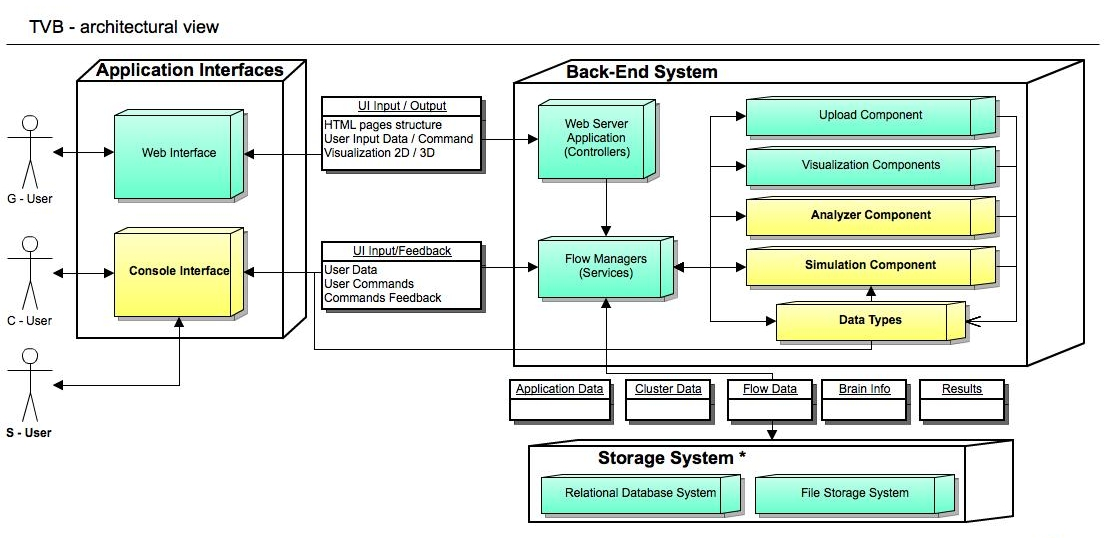
\includegraphics[width=0.90\textwidth]{images/architecture.jpg}
        \caption{TVB architecture: Yellow blocks are part of the Scientific
            Library of TVB, while the green blocks are part of TVB Framework.
            TVB provides two independent interfaces, depending on the
            interaction type wanted by the end-user (web or console).  TVB
            Storage layer is compulsory for the web interface, but it can be
            switched on/off for the console interface.  \note[lp]{It is said in
                the text that "console interface" is part of the "architecture"
            and not the "scientific library", this is the contrary on the
        figure}
        \note[lp]{What is a "S-User"? I missed the definition?}
         }
        \label{fig:architecture}
 \end{figure*}

 The goal of this article is firstly to decribre TVB framework from the
 development point of view and demonstrates how it interacts with other tools
 and how it can be extended (on the basis of extension already integrated in
 TVB).
